\chapter{泰勒定理及其应用}\label{ch:5}

泰勒公式是本册书前半部分的顶峰中的顶峰,是瑰宝,是仲夏夜的梦,是数学梦幻中的蠢蠢欲动。泰勒公式横盖前半学期所学知识,出现于各种习题,解决一切疑难杂症。或许在座的同学高中就听说过洛必达,但是洛必达的前方却是泰勒不朽的身影。所以各位同学一定要认真学好泰勒公式,现对本章脉络与重点说明如下:
\begin{enumerate}
	\item 明白泰勒公式出现的意义及其应用范围。
	\item 掌握泰勒公式基本形式以及对于典型函数的形式,麦克劳林展开式重中之重。
	\item 熟练在极限、不等式、证明、函数性态研究中应用泰勒公式。
\end{enumerate}

\section{背景:何来泰勒}\label{sec:5.1}

\subsection{泰勒出场的背景}\label{sec:5.1.1}

让我们回想一下在高中所学过的:一次、二次、三次、四次,五次函数的图像。
\begin{figure}[tbph]
	\centering
	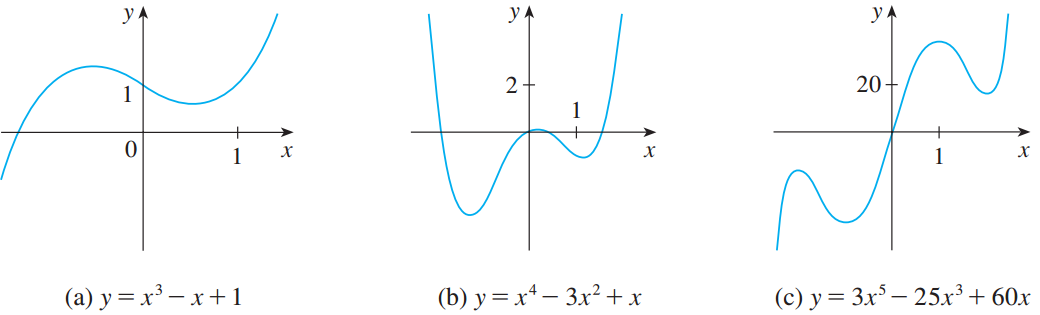
\includegraphics[width=0.7\linewidth]{figures/多项式函数图片}
	\caption{}
	\label{fig:5.1}
\end{figure}
此时我们发现,当多项书次数越高,函数所可以呈现的形状越多。

假设我们现在遇到了一个只知道函数表达式的函数,它的表达复杂诡异,求导的过程十分困难。

而为了实现对此函数的形态研究,我们就需要一个合适的$n$次多项式去拟合这个未知的函数,这就是泰勒出场的背景。

\subsection{从线性拟合到多项式拟合}\label{sec:5.1.2}
从第\ref{ch:3}章知道,对于极其靠近$x_0$的函数,我们用线性函数来近似表达
\begin{equation}
	f(x)\approx f(x_0)+f'(x_0)(x-x_0)\label{eq:5.1}
\end{equation}

那么对于某个区域$I$,需要用多项式去拟合,我们记此多项式为$P_n(x)$,则
\begin{equation}
	P_n(x)=a_0+a_1(x-x_0)+a_x(x-x_0)^2+...+a_n(x-x_0)^n\label{eq:5.2}
\end{equation}

如果实现
\begin{equation*}
	f(x)=P_n(x)+o\qty((x-x_0)^n)
\end{equation*}

即,误差为$(x-x_0)^n$的高阶无穷小,则实现了上述的拟合逼近。

那么如何寻找多项式的系数$a_n$呢\mn{使用牛顿插值法可以推导出泰勒公式的系数,有兴趣的同学自行查阅相关知识点。}?

\section{皮阿诺余项与拉格朗日余项的泰勒展开}

\subsection{带Peano余项的泰勒展开}
\begin{definition}
	\begin{equation}
		f(x)=\sum_{k=0}^n\frac{f^{(k)}(x_0)}{k!}(x-x_0)^k+o\qty((x-x_0)^n)\label{eq:5.3}
	\end{equation}

    像这样的展开称为带Peano余项的泰勒展开。
\end{definition}

此展开可以归结为以下形式:
$$
	f(x)=P_n(x)+R_n(x)
$$

其中,有
$$
P_n(x)=\sum\limits_{k=0}^n\frac{f^{(k)}(x_0)}{k!}(x-x_0)^k,R_n(x)=o((x-x_0)^n)
$$

此处$P_n(x)$称为泰勒多项式,系数称为泰勒系数;$R_n(x)$称为Peano余项,它们合称为带皮阿诺余项的泰勒展开。

\begin{remark}
	对于皮阿诺余项$R_n(x)$,仅能说明这个误差是$(x-x_0)^n)$的高阶无穷大小,不能对于误差大小作具体数值分析。而泰勒定理的另一种表达式,就可以解决这一问题。
\end{remark}

\subsection{带Lagrange余项的泰勒展开}\label{sec:5.2.2}

\begin{definition}
	\begin{equation}
		f(x)=\sum_{k=0}^n\frac{f^{(k)}(x_0)}{k!}(x-x_0)^k+\frac{f^{n+1}(\xi)}{(n+1)!}(x-x_0)^{n+1}\label{eq:5.4}
	\end{equation}

    像这样的展开称为带Lagrange余项的泰勒展开。
\end{definition}

此处$\frac{f^{n+1}(\xi)}{(n+1)!}(x-x_0)^{n+1}$称为拉格朗日余项,也可以写成如下形式:
$$
R_n(x)=\frac{f^{n+1}[x_0+\theta(x-x_0)]}{(n+1)!}(x-x_0)^{n+1},\theta\in(0,1)
$$

使用这一表达,我们就可以通过依据误差精度的需求来确定$n$的大小。

\section{Maclaurin公式}\label{sec:5.3}
学习了泰勒公式的形式之后,其实大家也能看出来,公式形式很复杂而且对于不同的场景有不同的适用情况。为了解决一部分问题,当采取了在0处进行展开的形式后,形成的公式形式方便记忆同时普适性强,我们称之为Maclaurin展开。基本形式如下:

\begin{equation}
    f(x)=f(0)+f'(0)x+\frac{f''(0)}{2!}+\frac{f'''(0)}{3!}+...+\frac{f^{n+1}(\theta x)}{(n+1)!}x^{n+1},~\theta\in(0,1)
    \label{eq:5.5}
\end{equation}

\subsection{需要记忆的常用展开}\label{sec:5.3.1}

\subsubsection{指数函数的展开($x\in(-\infty,+\infty),~\theta\in(0,1)$)}

\begin{equation}
	{\rm e}^x=1+x+\frac{x^2}{2!}+\frac{x^3}{3!}+\frac{x^4}{4!}+\cdots+\frac{x^n}{n!}+\frac{x^{n+1}}{(n+1)!}{\rm e}^{\theta x}\label{eq:5.6}
\end{equation}

\noindent\textbf{记忆技巧:}分子分母数字一致,全是加号。

\subsubsection{正弦函数的展开($x\in(-\infty,+\infty),~\theta\in(0,1)$)}
\begin{equation}
	\sin(x)=x-\frac{x^3}{3!}+\frac{x^5}{5!}-\frac{x^7}{7!}+\cdots+(-1)^{m-1}\frac{x^{2m-1}}{(2m-1))!}+(-1)^m\frac{\cos\theta x}{(2m+1)!}
	\label{eq:5.7}
\end{equation}

\noindent\textbf{记忆技巧:}纯奇数,正负正负交替。

\subsubsection{余弦函数的展开($x\in(-\infty,+\infty),~\theta\in(0,1)$)}
\begin{equation}
	\cos(x)=1-\frac{x^2}{2!}+\frac{x^4}{4!}-\frac{x^6}{6!}+\cdots+(-1)^m\frac{x^{2m}}{(2m)!}+(-1)^{m+1}\frac{\cos\theta x}{(2m+2)!}x^{2m+2}
	\label{eq:5.8}
\end{equation}
\noindent\textbf{记忆技巧:}纯偶数,依然是先正后负,正负正负交替。

\subsubsection{对数函数的展开($x\in(-1,+\infty),~\theta\in(0,1)$)}
\begin{equation}
	\ln(1+x)=x-\frac{x^2}{2}+\frac{x^3}{3}-\frac{x^4}{4}+\cdots+(-1)^{n-1}\frac{x^n}{n}+(-1)^n\frac{x^{n+1}}{(n+1)(1+\theta x)^{n+1}}
	\label{eq:5.9}
\end{equation}
\noindent\textbf{记忆技巧:}正负交替,不用阶乘。

\subsubsection{幂函数的展开($x\in(-1,\infty),\theta\in(0,1)$)}
\begin{equation}
	(1+x)^{\alpha}=1+\alpha x+\frac{\alpha(\alpha-1)}{2!}x^2+\cdots+\frac{\alpha(\alpha-1)\cdots(\alpha-n+1)}{n!}x^{n}+\frac{\alpha(\alpha-1)\cdots(\alpha-n)}{(n+1)!}\frac{x^{n+1}}{(1+\theta x)^{n+1-a}}
\end{equation}

\noindent\textbf{记忆技巧:}对于多项式部分,有$$P_n(x)=\frac{(\alpha)!}{(\alpha-n)!n!}x^n$$


\section{泰勒公式模型、套路、题型}

\subsection{泰勒公式的本质+如何选择Peano/Lagrange余项}
\subsubsection{泰勒公式的本质}
\begin{enumerate}
	\item 用多项式逼近函数。
	\item 用已知点信息表示未知点。
	\item 建立函数与高阶导数的关系。
\end{enumerate}

\subsubsection{如何选择Peano/Lagrange余项}
\begin{enumerate}
	\item 条件不同
	
	Peano:$f(x)$在点$x_0$处有至$n$阶的导数。
	
	Lagrange:$f(x)$在含有$x_0$的开区间$(a,b)$内有$n+1$阶的导数。
	
	\item 余项不同——应用场景不同
	
	Peano:局部的定性分析——求极限,极值
	
	Lagrange:整体的定量分析——求最值,不等式
\end{enumerate}

\subsection{泰勒公式求极限}
\subsubsection{应用泰勒公式统一为多项式}

\begin{problem}
	求$\lim\limits_{x\rightarrow 0}\frac{\cos(x)-{\rm e}^{-\frac{x^2}{2}}}{x^4}$。
	\begin{solution}
		$\cos(x)-{\rm e}^{-\frac{x^2}{2}}$都不好处理\mn{当你遇到极限而不得,如果形式混杂但是函数明晰,欢迎使用泰勒。},用\textbf{泰勒统一为多项式},取皮阿诺展开到与分母同阶或者比分母略高一阶即可。
		
		取Peano展开,$\cos(x)=1-\frac{x^2}{2!}+\frac{x^4}{4!}+o(x^5)$,${\rm e}^{-\frac{x^2}{2}}=1{-\frac{x^2}{2}}+\frac{\qty({-\dfrac{x^2}{2}})^2}{2!}+o_2(x^4)$,代入原式得
		\begin{equation*}
			\lim\limits_{x\rightarrow 0}\frac{1-\dfrac{x^2}{2!}+\dfrac{x^4}{4!}+o(x^5)-\qty[1-\dfrac{x^2}{2}+\dfrac{\qty(-\dfrac{x^2}{2})^2}{2!}+o_2(x^4)]}{x^4}=-\frac{1}{12}+\frac{o(x^4)}{x^4}=-\frac{1}{12}
		\end{equation*}
	\end{solution}
\end{problem}

\subsubsection{通过泰勒公式,从极限中研究函数}
\begin{problem}
	设$f(x)$在$x=0$的某邻域二阶可导,且$\lim\limits_{x\rightarrow 0}\qty(\frac{\sin 3x}{x^3}+\frac{f(x)}{x^2})=0$,则\xparen
	\begin{xchoices}[showanswer=true]
		\item $\lim\limits_{x\rightarrow 0}\qty(\frac{3}{x^2}+\frac{f(x)}{x^2})=0$
		\item $f(0)=3$
		\item $f'(0)=3$
		\item* $f''(0)=9$
	\end{xchoices}
    \vspace{0.5em}
    \begin{solution}
    	这是一个披着极限的外衣,让我们研究函数性态的习题。
    	
    	原式改写为$$\lim\limits_{x\rightarrow 0}\frac{\dfrac{\sin 3x}{x}+f(0)+f'(0)x+\dfrac{f''(0)}{2}x^2+o(x^2)}{x^2}$$
    	
    	注意虽然$\lim\limits_{x\rightarrow 0}\frac{\sin 3x}{x}=3$,但是因为此式下面还有一个$x^2$,所以需要用泰勒改写为$\sin 3x=3x-\frac{(3x)^3}{3!}$,故原式为$$\lim\limits_{x\rightarrow 0}\frac{3-\dfrac{27}{6x^2}+f(0)+f'(0)x+\dfrac{f''(0)}{2}x^2+o(x^2)}{x^2}=0$$
    	
    	则
    	$$\lim\limits_{x\rightarrow 0}\qty[-\frac{9}{2}+\frac{(f(0)+3)+f'(0)x+\dfrac{f''(0)}{2}x^2+o(x^2)}{x^2}]=0$$
    	
    	故\mn{这就是通过极限的必要条件,对于函数性态的研究。}$$f(0)=-3,f'(0)=0,f''(0)=9$$
    \end{solution}
\end{problem}

\begin{problem}
	设$y=f(x)\mbox{在}(-1,1)$内具有二阶连续导数,且$f''(x)\neq 0$,试证:
	\begin{enumerate}[label=(\arabic*)]
		\item 对于$(-1,1)$内的任一$x\neq 0$,存在唯一的$\theta x\in(0,1)$,使$$f(x)=f(0)+xf'\qty(\theta(x)x)$$成立;
		\item  $\lim\limits_{x\rightarrow 0}\theta(x)=\frac{1}{2}$。
	\end{enumerate}
    \begin{proof}
    	\begin{enumerate}[label=(\arabic*)]
    		\item 即证明拉格朗日中值定理在题设条件下的唯一性。
    		
    		由拉格朗日中值定理,得到\mn{这里面的$\theta(x)$表明$\theta$是$x$的函数,没有其他意思}$$f(x)=f(0)+xf\qty(\theta(x)x),~\theta(x)\in(0,1)$$
    		
    		由$f''(x)\neq 0$,得到导函数单调减或者单调增,$\theta$唯一。
    		\item  属于泰勒的变形,十分需要记忆。
    		
    		由二阶可导得$$f(x)=f(0)+f'(0)x+\frac{1}{2}f'(\xi)x^2$$所以$xf\qty(\theta(x)x)=f'(0)+
    		\frac{1}{2}f''(\xi)x^2$,从而$$\lim\limits_{x\rightarrow 0}\theta(x)\frac{f'(\theta(x)x)-f'(0)}{\theta(x)x}=\lim\limits_{x\rightarrow 0}\frac{1}{2}f''(\xi)=\lim\limits_{x\rightarrow 0}\frac{1}{2}f''(0)=\lim\limits_{x\rightarrow 0}\theta(x)f''(0)$$
    		故\mn{见到题设条件又二阶连续导数,某个函数不等于0,要注意应用条件,不要忽略。}$\lim\limits_{x\rightarrow 0}\theta(x)=\frac{1}{2}$
    	\end{enumerate}
    \end{proof}
\end{problem}

\subsection{泰勒公式求解函数性态}
\subsubsection{泰勒公式求解函数最值}
\begin{problem}
	设函数$f(x)$在$[0,1]$上二阶可导,且$f(0)=1,f'(0)=0,f''(1)\leq 1$,试证$f(x)$在$[0,1]$上的最大值不超过$\frac{3}{2}$。
	\begin{solution}
		由于题目中的函数二阶可导,所以泰勒也只能写到二阶\mn{利用泰勒拟合函数,通过已知条件进行放缩。}。
		$$f(x)=1+\frac{f''(\xi)}{2!}x^2\neq 1+\frac{x^2}{2}\leq\frac{3}{2}$$
	\end{solution}
\end{problem}

\subsubsection{泰勒公式求解高阶导数}
\begin{problem}
	求$f(x)=x^2\cdot2^x$在$x=0$处的$n$阶导数$f^n(0)$。
	\begin{solution}
		很显然,如果用泰勒展开成多项式,小于n次方的项求导后消失,大于$n$次方的求导后为0,这也太棒了。
		
		$$f(x)=x^2\cdot2^x=x^2\qty[1+x\ln2+\cdots+\frac{(\ln2)^nx^n}{n!}+o(x^n)]$$
		
		故$x^n$项的系数是$a_n=\frac{(\ln2)^{n-2}}{(n-2)!}$,而$f^n(0)=n!a_n$,故$f^n(0)=n(n-1)(\ln2)^{n-2}$
	\end{solution}
\end{problem}

\subsection{泰勒公式证明不等式}
\begin{problem}
    设$f''(x)>0$,当$x\rightarrow 0$时,$f(x)$和$x$是等价无穷小。证明:当$x\neq 0$时$f(x)>x$。
	\begin{proof}
		由于题目中的函数二阶可导\mn{当出现二阶导数的情况,我们常选用泰勒确定函数性态。},所以泰勒也只能写到二阶。由题意,得到$f(0)=0$,$f'(0)=1$
		$$f(x)=f(0)+f'(0)x+\frac{f''(\xi)}{2!}x^2=x+\frac{f''(\xi)}{2!}x^2>x$$
	\end{proof}
\end{problem}